\chapter{基于变量消除的精确推断}
\label{chap:pgm-elimination}

前四章解决的是“怎样表示”一个概率模型：给定图和局部因子，联合分布被写成一组局部函数的乘积。从本章开始进入第二部分，要回答表示之后最自然的问题——模型已经建好，怎样用它回答具体查询？这就是\term{推断}（inference）。设备报警后，维修人员面对的诊断任务通常有两种输出：一种是给出故障的后验概率，回答“有多可能是故障”；另一种是直接选出一组最可能的故障、过热和传感器状态，回答“最可能是什么情形”。这两种输出使用同一组局部因子，区别只在于用什么方式汇总那些没有观测到、也不要求作答的状态。

先看最朴素的做法为什么不够。要计算一个后验概率，原则上可以列出所有变量的完整联合配置，把符合查询和证据的配置权重逐一相加。但对$d$个二元变量，完整配置有$2^d$个：$d=30$时就超过十亿，变量再多便完全不可行。联合分布写成局部因子乘积的意义正在于避免这种指数级的整体枚举——许多局部和与查询变量无关，可以先算一次、再被多个查询配置重复使用。利用局部分解识别并消除这些重复计算，正是精确推断的主要任务。本章从第~\ref{sec:pgm-representations-local-computation}节已经引入的因子组合与消元操作出发，把它发展成完整、可证明正确的算法。

核心想法是逐个处理未知变量，而不是一次处理全部。查询通常只保留部分变量，某个未知变量对答案的全部影响，可以先汇总成一个只依赖剩余变量的更小函数，供后续步骤重复使用。\term{变量消除}（variable elimination, VE）据此逐个收集含有当前变量的因子。本步收集到的这些因子称为当前变量的\term{桶}（bucket）——之所以必须一起处理，是因为它们要使用当前变量的同一个状态，不能各自独立求和。将桶内因子相乘，再以求和、积分或最大化消去该变量，所得新函数便可替换桶内函数，保存它们对剩余变量的共同影响。

本章围绕三个问题展开：其一，为什么这样逐桶替换不会改变最终的查询答案，这需要一个贯穿全章的不变式来证明；其二，不同查询（求概率、求最可能完整配置、求部分变量的最优值）为什么要选用求和或最大化等不同算子，以及这些算子能否交换次序；其三，消元顺序怎样改变中间函数的作用域，从而决定计算量。离散因子以状态组合数表示规模，高斯因子则以矩阵块维度表示规模，两种表示由此产生不同的计算代价。

\section{推断问题与因子运算}
\label{sec:pgm-elimination-factor-operations}

\subsection{查询、证据与消元变量}
\label{sec:pgm-elimination-query-evidence}

在给出算法前，先把一个推断查询涉及的变量角色固定下来，这是后面所有记号的基础。求故障后验时，要固定报警证据，保留故障变量作为查询目标，并把其余未知状态全部汇总掉。一般地，模型的节点集合为$V$，节点$i$对应随机变量$X_i$；已观测节点组成$O\subseteq V$，取值为$\bm{x}_O=\bm{e}$，查询节点组成$Q\subseteq V\setminus O$。剩下既未观测、也不查询的节点称为待消元节点，记为$R=V\setminus(O\cup Q)$——它们的值不是答案，但它们的各种取值都会影响答案，需要被汇总。三个大写集合指定变量角色，$\bm{x}_Q$才是一组查询状态。证据集合用$O$记，以便与图的边集合$E$区分。

以下把模型参数视为已知输入。设共有$m$个非负因子$\psi_a$，其完整乘积具有有限且非零的归一化常数$Z$，联合分布写为
\begin{equation}
  p(\bm{x})=\frac{1}{Z}\prod_{a=1}^{m}\psi_a(\bm{x}_{S_a}),
  \qquad S_a\subseteq V.
  \label{eq:pgm-elimination-factorization}
\end{equation}
有向模型采用局部条件概率作为因子，完整积已归一化，故$Z=1$。无向模型的势需由全局$Z$归一化。这些函数都是当前推断的输入，第~\ref{chap:pgm-parameter-learning}章再讨论如何从数据估计它们。

把证据坐标固定在观测值后，原乘积成为未观测变量上的函数：
\begin{equation}
  F_{\bm{e}}(\bm{x}_{V\setminus O})
  =\left.\prod_{a=1}^{m}\psi_a(\bm{x}_{S_a})
  \right|_{\bm{x}_O=\bm{e}}.
  \label{eq:pgm-elimination-evidence-function}
\end{equation}
先取各变量状态数有限的离散情形。汇总$R$的联合状态得到查询权重，再对$Q$的所有状态归一化：
\begin{equation}
  \begin{aligned}
    g_Q(\bm{x}_Q)
      &=\sum_{\bm{x}_R}F_{\bm{e}}(\bm{x}_Q,\bm{x}_R),\\
    Z_{\bm{e}}&=\sum_{\bm{x}_Q}g_Q(\bm{x}_Q),\\
    p(\bm{x}_Q\mid\bm{e})&=\frac{g_Q(\bm{x}_Q)}{Z_{\bm{e}}}.
  \end{aligned}
  \label{eq:pgm-elimination-marginal-query}
\end{equation}
下标$\bm{x}_R$遍历待消元变量的联合状态。这里值得指出一个在实现上很方便的事实：总权重满足$Z_{\bm{e}}=Zp(\bm{e})$，因此计算条件概率时，无向模型那个麻烦的全局归一化常数$Z$会在分子分母中直接抵消。也就是说，无论模型有没有写出$Z$，推断都可以直接从未归一化的因子乘积出发，最后只做一次归一化。后验比值在$Z_{\bm{e}}>0$的证据事件上有定义；模型赋予观测零概率时，该比值的分母为零，此时条件分布本身没有定义。

连续变量用积分汇总未知坐标。联合密度存在且积分有限时，式~\eqref{eq:pgm-elimination-marginal-query}的积分版本给出边缘条件密度。连续观测处的$p(\bm{e})$表示边缘密度值，比值只在密度有限且为正的观测处使用。形式相同的查询还需配合适当的函数表示，才能解析完成积分。

\subsection{因子乘积}
\label{sec:pgm-elimination-factor-product}

变量消除每一步都在对因子做三种基本操作：相乘、按证据切片、对未知变量求和。这三种操作各自改变因子的不同坐标，后续算法会反复使用它们。

相乘两张因子表时，需要按变量身份及状态含义对齐坐标。\term{作用域}（scope）指定因子的自变量。一次消元先合并相关因子的作用域，再从中去掉本次被消去的变量，余下坐标就是新因子需要保留的输入。若$D_i$是$X_i$的取值集合，作用域为$S$的离散因子是非负函数$\psi_S:\prod_{i\in S}D_i\to[0,\infty)$。存储表时还要记下$S$内变量的排列和状态编码：同一变量可以位于不同表轴上，但相乘时同一个状态必须有相同含义。

两个函数分别使用$A$与$B$中的变量，乘积便使用它们的并集$A\cup B$：
\begin{equation}
  (\psi_A\psi_B)(\bm{x}_{A\cup B})
  =\psi_A(\bm{x}_A)\psi_B(\bm{x}_B).
  \label{eq:pgm-elimination-product}
\end{equation}
对$A\cup B$的一组取值，两因子各读取自己的坐标，其中共享变量取同一状态。例如，$\psi_{\{F,H\}}(f,h)\psi_{\{H,S\}}(h,s)$以$(f,h,s)$为索引；计算$(0,1,0)$时，分别读取前表$(0,1)$与后表$(1,0)$。三个变量均为二元时，两张$4$项表的乘积共有$8$项，新增的坐标来自两表作用域的并集。

因子保存相对权重，其全表求和可以异于$1$。空作用域的因子是标量，也参与完整乘积；条件概率比较中的公共尺度可约去，而证据概率或绝对得分需要这些尺度。乘积还要保留函数的出现次数：两个数值相同的因子仍相乘两次。以下的$\mathcal{F}$因此按多重集合使用。

\subsection{因子约简与边缘化}
\label{sec:pgm-elimination-reduction-marginalization}

观测把一个变量的状态固定后，可以从因子表读取相应切片。把证据代入并从作用域移去固定坐标，称为\term{因子约简}（factor reduction）。报警证据$A=1$将$p(a\mid h,s)$变为$\ell_A(h,s)=p(A=1\mid h,s)$，表示各$(h,s)$状态对该报警的支持权重。结合先验与其他因子、再统一归一化，才能得到这些原因的后验分布。

对状态仍未知的变量，概率查询要汇总其全部取值。\term{边缘化}（marginalization）把这些权重相加，留下其余坐标上的函数：若$i\in S$，则
\begin{equation}
  (\mathop{\textstyle\sum}_{x_i}\psi_S)
    (\bm{x}_{S\setminus\{i\}})
  =\sum_{x_i\in D_i}\psi_S(\bm{x}_{S\setminus\{i\}},x_i).
  \label{eq:pgm-elimination-factor-marginal}
\end{equation}
约简读取已知状态下的切片，边缘化累加未知状态。两种操作都减少自变量数，分别保留观测条件下的权重与未知变量的总贡献。

一个未知变量可能同时出现在多个因子中，这时汇总的次序至关重要：必须让这些因子共享$X_i$的同一个状态。若$X_i$同时出现在$\psi_1(x_i,y)$和$\psi_2(x_i,z)$中，正确做法是先相乘、再对共同的$x_i$求和，所得新因子为
\[
  \sum_{x_i}\psi_1(x_i,y)\psi_2(x_i,z)\text{。}
\]
反过来，若先各自对$x_i$求和再相乘，相当于允许第一张表选定的$x_i$取值与第二张表选定的取值彼此独立、互不相同，这就破坏了“同一个$x_i$”的约束，得到的是另一个量。因此，消元必须先收集所有含$X_i$的因子、把它们乘在一起，再对共同乘积汇总；新函数保留的是这些因子在剩余坐标上的联合影响。这也解释了“桶”为什么要成组处理，而不能逐因子独立求和。

完成非查询变量的边缘化后，查询权重可以统一归一化。中途若用一个与全部自变量无关的正常数缩放因子，最终条件概率的公共尺度仍会抵消，但计算$Z_{\bm{e}}$需记录并补回该常数。逐行归一化的除数随剩余坐标变化，会改变各查询配置的相对权重，因而属于对函数的实质修改。

\section{边缘概率的变量消除算法}
\label{sec:pgm-elimination-sum-product}

这一节用一个可以逐项手算的小模型，看清变量消除究竟省下了什么，再把其中的规则提炼成一般算法。故障后验要把所有非查询状态的权重相加，因此这里使用求和消元。我们先在报警模型上比较完整枚举与局部汇总，找出能够重复使用的子计算，再把相同规则写成一般算法。保留多个查询变量时，汇总规则不变，改变的是输出函数的坐标；连续变量则把求和换成积分，还需选择能够精确保存积分结果的函数表示。

\subsection{从朴素枚举到分配律}
\label{sec:pgm-elimination-distributivity}

沿用报警模型作为可逐项计算的例子：故障$F$、过热$H$、报警$A$和传感器失灵$S$均取$0$或$1$。联合分解为
\begin{equation}
  p(f,h,a,s)=p(f)p(h\mid f)p(s)p(a\mid h,s).
  \label{eq:pgm-elimination-alarm-model}
\end{equation}
有向结构$F\to H\to A\leftarrow S$使两个根节点$F,S$独立。设置$p(F=1)=0.1$、$p(S=1)=0.05$，并取
\[
  p(H=1\mid F=0)=0.1,\qquad
  p(H=1\mid F=1)=0.8.
\]
表~\ref{tab:pgm-elimination-alarm-cpt}给出四种$(h,s)$下的报警概率；二元分布的状态$0$概率都由$1$减去状态$1$概率得到。这组人工参数只用于解释消元步骤。

\begin{table}[htbp]
  \centering
  \begin{tabular}{ccc}
    \toprule
    $h$ & $s$ & $p(A=1\mid h,s)$\\
    \midrule
    $0$ & $0$ & $0.01$\\
    $1$ & $0$ & $0.90$\\
    $0$ & $1$ & $0.70$\\
    $1$ & $1$ & $0.99$\\
    \bottomrule
  \end{tabular}
  \caption{报警模型的人工条件表。每行固定$(h,s)$并列出$p(A=1\mid h,s)$，同一行的不报警概率为$1-p(A=1\mid h,s)$。}
  \label{tab:pgm-elimination-alarm-cpt}
\end{table}

将$A=1$代入报警因子后，故障查询需要累加过热和传感器的全部状态：
\[
  g_F(f)=\sum_h\sum_s p(f)p(h\mid f)p(s)\ell_A(h,s).
\]
直接枚举对每个$f$访问全部$(h,s)$，共需访问$8$个三元配置。仔细观察会发现，其中$p(s)\ell_A(h,s)$这部分完全不含$f$：无论查询的是$f=0$还是$f=1$，它都要被计算同样一遍。让两种故障状态共享这部分结果，就能避免重复。利用乘法对加法的分配律（先对与当前变量无关的因子求和，再乘回相关因子，结果不变），先对$s$汇总与它相关的两个函数：
\begin{equation}
  g_F(f)
  =p(f)\sum_h p(h\mid f)
    \underbrace{\sum_s p(s)\ell_A(h,s)}_{\tau_S(h)}.
  \label{eq:pgm-elimination-alarm-reorder}
\end{equation}
所得$\tau_S(h)$替换$p(s)$与$\ell_A(h,s)$，对每种$h$计算一次，供所有$f$使用。下一步将$p(h\mid f)\tau_S(h)$对$h$求和，生成$f$上的函数。图~\ref{fig:pgm-elimination-alarm-buckets}将每步输入与输出的坐标分别画出。

\begin{figure}[htbp]
  \centering
  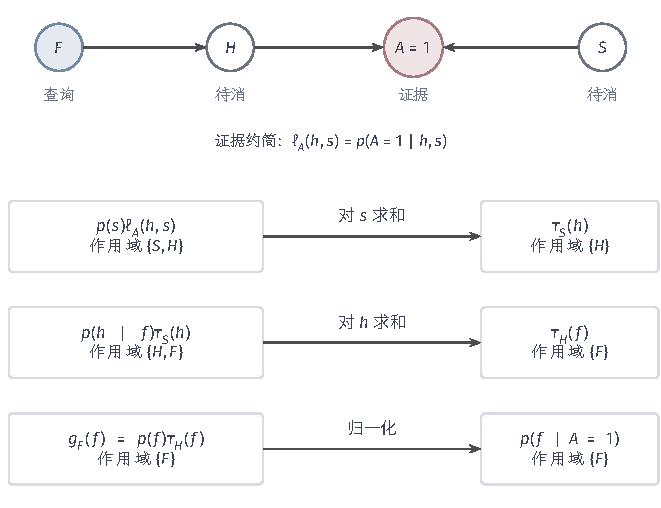
\includegraphics[width=112.000mm]{figures/09-probabilistic-graphical-models/02-inference/tikz/pgm-elimination-alarm-buckets/figure.pdf}
  \caption{故障后验查询的两步消元。上方有向图中，蓝色$F$为查询变量，红色$A=1$为证据，灰边空心的$H,S$为待消变量。下方先从$p(s)\ell_A(h,s)$求和得到$\tau_S(h)$，再从$p(h\mid f)\tau_S(h)$求和得到$\tau_H(f)$。每步输出的作用域只保留尚未消去的坐标；最终将$g_F(f)=p(f)\tau_H(f)$按$f$归一化，得到$p(f\mid A=1)$。}
  \label{fig:pgm-elimination-alarm-buckets}
\end{figure}

这种重排让后续故障状态复用同一局部汇总，每个$s,h$状态仍以原权重参与求和，所以代数结果与完整枚举相同——这正是“消除”而非“近似”的含义：它只改变求和的组织次序，不改变任何一项的贡献。能省多少取决于输出函数的作用域：新表只涉及剩余变量，若一桶包含几乎全部剩余变量，形成的新表仍可能很大。选择消元顺序的目的，就是控制这类中间函数的坐标数和状态组合数，这是第~\ref{sec:pgm-elimination-complexity}节的主题。

\subsection{变量消除算法}
\label{sec:pgm-elimination-ve-algorithm}

一般因子分解也按同一方式替换局部乘积。证据约简后的初始因子多重集合记为$\mathcal{F}^{(0)}$，顺序$\pi=(i_1,\ldots,i_k)$将待消元集合$R$的每个节点列出恰好一次。第$t$步收集全部含$X_{i_t}$的因子：
\[
  \mathcal{B}_t
  =\{\psi\in\mathcal{F}^{(t-1)}:
      i_t\in\operatorname{scope}(\psi)\}.
\]
$\operatorname{scope}(\psi)$给出函数的作用域。前面所说的变量的桶，现在由多重集合$\mathcal{B}_t$准确记录，其中的函数需要共同参与本步求和。令$U_t$为它们作用域的并集，去掉当前变量后的集合为$N_t=U_t\setminus\{i_t\}$，局部更新写为
\begin{equation}
  \begin{aligned}
    \phi_t(\bm{x}_{U_t})&=\prod_{\psi\in\mathcal{B}_t}\psi,\\
    \tau_t(\bm{x}_{N_t})&=\sum_{x_{i_t}}\phi_t(\bm{x}_{U_t}).
  \end{aligned}
  \label{eq:pgm-elimination-local-sum}
\end{equation}
计算$\phi_t$时，先按式~\eqref{eq:pgm-elimination-product}对齐每个函数的坐标。桶外函数不含$X_{i_t}$，从本步求和提出后仍留在当前集合中。

\begin{algorithm}[离散边缘概率的变量消除]
  \label{alg:pgm-elimination-marginal}
  \begin{algorithmic}[1]
    \Require 取有限非负值的离散因子$\{\psi_a\}$，证据$\bm{x}_O=\bm{e}$，查询集$Q$
    \Require $R=V\setminus(O\cup Q)$的排列$\pi=(i_1,\ldots,i_k)$
    \Ensure 查询因子$g_Q$及$Z_{\bm{e}}>0$时的条件分布
    \State 将证据代入各因子，得到$\mathcal{F}^{(0)}$；保留标量因子
    \State 对未出现在任何作用域中的未观测变量，加入其恒为$1$的一元因子
    \For{$t=1,\ldots,k$}
      \State 收集$\mathcal{B}_t$，令$U_t$为其作用域的并集
      \State 对齐坐标并求乘积$\phi_t=\prod_{\psi\in\mathcal{B}_t}\psi$
      \State 对$x_{i_t}$求和，得到$\tau_t(\bm{x}_{U_t\setminus\{i_t\}})$
      \State $\mathcal{F}^{(t)}\gets
        (\mathcal{F}^{(t-1)}\setminus\mathcal{B}_t)\cup\{\tau_t\}$
    \EndFor
    \State 在查询取值空间上计算$g_Q=\prod_{\psi\in\mathcal{F}^{(k)}}\psi$
    \State 计算$Z_{\bm{e}}=\sum_{\bm{x}_Q}g_Q(\bm{x}_Q)$
    \If{$Z_{\bm{e}}=0$}
      \State 返回证据与模型不相容，条件分布未定义
    \Else
      \State 返回$g_Q$、$Z_{\bm{e}}$及$g_Q/Z_{\bm{e}}$
    \EndIf
  \end{algorithmic}
\end{algorithm}

算法~\ref{alg:pgm-elimination-marginal}按出现次数移除桶内函数并加入新因子。若某个未观测变量未进入任何函数，加入恒为$1$的一元因子后，它的求和仍贡献状态数。$R=\varnothing$时没有消元步骤，$Q=\varnothing$时最终乘积是证据权重标量$Z_{\bm{e}}$。边缘查询输出汇总后的函数，各个已消变量的状态都参与了累加，因此输出无需配置回溯。

报警例的数值虽然小，却能完整展示算法每一步。报警查询从$p(f)$、$p(h\mid f)$、$p(s)$和$\ell_A(h,s)$四因子开始。先处理$S$桶：$p(s)$与$\ell_A(h,s)$相乘后对$s$求和，两种$h$下的新函数值分别为
\begin{equation}
  \begin{aligned}
    \tau_S(0)&=0.95\times0.01+0.05\times0.70=0.0445,\\
    \tau_S(1)&=0.95\times0.90+0.05\times0.99=0.9045.
  \end{aligned}
  \label{eq:pgm-elimination-alarm-s}
\end{equation}
用$\tau_S(h)$替换$S$桶后，当前集合为$\{p(f),p(h\mid f),\tau_S(h)\}$。接着将含$H$的两个函数相乘并求和，得到
\begin{equation}
  \begin{aligned}
    \tau_H(0)&=0.9\times0.0445+0.1\times0.9045=0.1305,\\
    \tau_H(1)&=0.2\times0.0445+0.8\times0.9045=0.7325.
  \end{aligned}
  \label{eq:pgm-elimination-alarm-h}
\end{equation}
余下$p(f)$与$\tau_H(f)$相乘，给出$g_F(0)=0.11745$、$g_F(1)=0.07325$，总权重为$0.19070$。原有向联合积的$Z=1$，因此此值也是证据概率$p(A=1)$。把故障状态$1$的权重除以总权重，得到
\begin{equation}
  p(F=1\mid A=1)
  =\frac{0.07325}{0.19070}
  \approx0.384111.
  \label{eq:pgm-elimination-alarm-posterior}
\end{equation}
报警使故障概率从$0.1$升至约$0.384$。无故障过热、传感器失灵以及小概率误报也能解释报警，它们的概率都进入求和分母；保留这些解释使后验仍低于$1$。

这个顺序只产生$\tau_S(h)$、$\tau_H(f)$两张一元表。变量较多的模型可先按消元顺序分桶。对一个输入因子，先看它的作用域是否含有待消元节点：若含有，就交给顺序中最早的那个节点；若只含查询节点，就放入最终查询因子池，留到所有桶处理结束后再相乘。空作用域的标量因子也保留在最终池中，使绝对证据权重不丢失。

每步新函数也按同一规则交接：仍含尚未消去的节点时，送往其中最早的后续桶；只剩查询坐标或成为标量时，放入最终池。当前报警查询中，$p(f)$从开始便留在最终池，$\tau_S(h)$送往$H$桶，最后生成的$\tau_H(f)$才汇入最终池。两者相乘得到$g_F(f)$，与算法~\ref{alg:pgm-elimination-marginal}保留当前因子集合再取积的做法一致。这种收集、合并、汇总的组织方式对应Dechter的桶消除算法\scite{pgm-elimination-dechter1999}

\subsection{多变量查询}
\label{sec:pgm-elimination-multivariate-query}

联合查询故障与传感器状态时，保留$Q=\{F,S\}$，仅消去$H$。所需结果使用$(f,s)$共同索引：
\begin{equation}
  g_{F,S}(f,s)
  =p(f)p(s)\sum_h p(h\mid f)\ell_A(h,s).
  \label{eq:pgm-elimination-joint-query}
\end{equation}
以$f=s=0$为例，先汇总两种过热状态，得到
\[
  \begin{aligned}
    g_{F,S}(0,0)
    &=0.9\times0.95\times(0.9\times0.01+0.1\times0.90)\\
    &=0.084645.
  \end{aligned}
\]
对其余三种$(f,s)$执行相同求和，即得到表~\ref{tab:pgm-elimination-joint-query}。

\begin{table}[htbp]
  \centering
  \begin{tabular}{ccc}
    \toprule
    $f$ & $g_{F,S}(f,0)$ & $g_{F,S}(f,1)$\\
    \midrule
    $0$ & $0.084645$ & $0.032805$\\
    $1$ & $0.068590$ & $0.004660$\\
    \bottomrule
  \end{tabular}
  \caption{报警证据下的未归一化$(F,S)$联合权重。四项共用归一化常数$0.19070$，得到$p(f,s\mid A=1)$；若各行分别归一化，则得到给定$f$后的传感器条件分布。}
  \label{tab:pgm-elimination-joint-query}
\end{table}

四项总权重为$0.19070$，各行之和是$g_F(f)$，各列之和是$g_S(s)$。虽然$F,S$观测前独立，报警后的两种原因相互影响：一种解释的后验权重会改变另一种解释的相对可信度。联合表保留了这种关系，两个一元后验的乘积一般给不出它。显式联合输出还有自身的存储代价；保留的查询变量越多，即使各消元桶较小，最后的联合表也可能很大。

\subsection{连续变量的边缘消除}
\label{sec:pgm-elimination-gaussian}

连续变量（如温度、测量值）的推断思路完全一样：先把涉及同一变量的因子相乘，再对它积分；不含当前坐标的因子可以提出积分号，非负可测性允许按Tonelli定理交换积分次序。条件密度还要求总积分有限且为正。但离散情形里“对有限状态求和”总是可以逐项完成并精确保存，连续情形则多了一个表示问题：积分后的函数未必还能用有限个参数精确表达。例如对任意形状的势做积分，结果可能是一个没有简单闭式的函数。因此能否解析消元，取决于因子的函数形式。高斯分布的二次指数形式恰好具有一个好性质：高斯函数相乘、以及在合法条件下积分，结果仍然是高斯二次指数。它因此提供了一个可以完整、精确计算的连续例子，本节就以它说明连续消元的参数如何更新。

高斯核的自变量记为$\bm{x}\in\mathbb{R}^{q}$。将其写成\term{规范形式}（canonical form），以二次项、一次项及常数项系数保存函数，便于相乘时合并参数：
\begin{equation}
  \psi(\bm{x})
  =\exp\!\left\{-\frac12\bm{x}^{\top}\bm{J}\bm{x}
                  +\bm{h}^{\top}\bm{x}+c\right\}
  \text{。}
  \label{eq:pgm-elimination-gaussian-canonical}
\end{equation}
参数$\bm{J}\in\mathbb{R}^{q\times q}$对称，$\bm{h}\in\mathbb{R}^{q}$，$c$为标量。对均值$\bm{\mu}$、协方差$\bm{\Sigma}$的非退化高斯密度，\term{精度矩阵}（precision matrix）$\bm{J}=\bm{\Sigma}^{-1}$以逆协方差表示二次项，$\bm{h}=\bm{J}\bm{\mu}$，归一化常数进入$c$。局部因子可以在部分方向没有二次约束；所有因子组合后的联合精度要求正定，使完整高斯核可归一化。以下用同样的三参数形式保存局部函数，但只对可归一化的完整核将其二次项矩阵解释为概率分布的精度。

规范形式相乘会将指数相加，因此对齐坐标后分别累加$\bm{J}$、$\bm{h}$和$c$即可。不在某因子作用域内的坐标补零，与离散表相乘时扩展坐标的操作对应。吸收证据仍是代入，不过观测坐标还会通过交叉二次项改变保留坐标的一次项。将当前函数的坐标分为保留块$\bm{x}_A$和观测块$\bm{x}_O=\bm{e}$，我们先把代入后的指数完整写出：
\[
  \begin{aligned}
    &-\frac12\bm{x}_A^{\top}\bm{J}_{A,A}\bm{x}_A
      -\frac12\bm{x}_A^{\top}\bm{J}_{A,O}\bm{e}
      -\frac12\bm{e}^{\top}\bm{J}_{O,A}\bm{x}_A\\
    &\quad-\frac12\bm{e}^{\top}\bm{J}_{O,O}\bm{e}
      +\bm{h}_A^{\top}\bm{x}_A+\bm{h}_O^{\top}\bm{e}+c
      \text{。}
  \end{aligned}
\]
由于$\bm{J}$对称，两个交叉项是相同的标量，合起来为$-\bm{x}_A^{\top}\bm{J}_{A,O}\bm{e}$。它对$\bm{x}_A$是一次项；只含$\bm{e}$的部分则与保留坐标无关，进入常数项。按这三类项读取系数，得到约简后的参数：
\[
  \begin{aligned}
    \bm{J}'&=\bm{J}_{A,A},\\
    \bm{h}'&=\bm{h}_A-\bm{J}_{A,O}\bm{e},\\
    c'&=c+\bm{h}_O^{\top}\bm{e}
       -\frac12\bm{e}^{\top}\bm{J}_{O,O}\bm{e}
       \text{。}
  \end{aligned}
\]
这组参数保存固定$\bm{x}_O$后的函数，未观测变量仍全部保留。接下来积分消元才汇总未知坐标的贡献。

一次积分先收集所有含待消变量的因子，将桶积写成式~\eqref{eq:pgm-elimination-gaussian-canonical}。作用域分为待消块$B$和保留块$A$，令$\bm{y}=\bm{x}_B\in\mathbb{R}^{b}$、$\bm{z}=\bm{x}_A\in\mathbb{R}^{a}$，相应参数为
\[
  \bm{J}=
  \begin{pmatrix}
    \bm{J}_{B,B}&\bm{J}_{B,A}\\
    \bm{J}_{A,B}&\bm{J}_{A,A}
  \end{pmatrix},
  \qquad
  \bm{h}=
  \begin{pmatrix}\bm{h}_B\\\bm{h}_A\end{pmatrix}
  \text{。}
\]
这里的$\bm{J}$和$\bm{h}$只来自当前桶。为区分局部函数与完整当前乘积，另以$T$表示当前尚未消去的全部节点，以$\bm{K}$和$\bm{\eta}$分别表示完整乘积的二次项和一次项参数。令$C=T\setminus B$为积分后全部剩余坐标；本桶的保留集$A$只是$C$的子集。桶外函数不含$\bm{y}$，因此它们不向$B,B$块贡献二次项，完整矩阵满足$\bm{K}_{B,B}=\bm{J}_{B,B}$。同样，$\bm{K}_{B,C}$由$\bm{J}_{B,A}$在$C$中其余坐标处补零得到。

关于$\bm{y}$的积分使用正定主块$\bm{J}_{B,B}\succ0$。非退化联合高斯模型的完整精度正定；证据约简后取相应主块仍然正定。若完整当前精度$\bm{K}\succ0$，它的主块$\bm{K}_{B,B}$正定，所以上述相等关系保证本桶满足积分条件。下面还会证明，完整边缘核的更新矩阵继续正定，因而这一条件可以逐步保持。这里要求正定的是被积分的主块；整个局部桶矩阵$\bm{J}$可以在其它方向没有约束。

为了计算一次积分，我们先从指数中提取含$\bm{y}$的项。利用$\bm{J}_{A,B}=\bm{J}_{B,A}^{\top}$合并交叉项，得到
\[
  -\frac12\bm{y}^{\top}\bm{J}_{B,B}\bm{y}
  +\bm{y}^{\top}(\bm{h}_B-\bm{J}_{B,A}\bm{z})
  \text{。}
\]
未写入这一行的保留项为$-\bm{z}^{\top}\bm{J}_{A,A}\bm{z}/2+\bm{h}_A^{\top}\bm{z}+c$。这些项与$\bm{y}$无关，所以它们对应的指数函数可以提出积分号，但仍须乘在积分结果上。将线性系数记为$\bm{u}(\bm{z})=\bm{h}_B-\bm{J}_{B,A}\bm{z}$。对$\bm{y}$配方，可以分离需要积分的高斯核与保留的$\bm{z}$函数：
\begin{equation}
  \begin{aligned}
    &-\frac12
      \bigl(\bm{y}-\bm{J}_{B,B}^{-1}\bm{u}\bigr)^{\top}
      \bm{J}_{B,B}
      \bigl(\bm{y}-\bm{J}_{B,B}^{-1}\bm{u}\bigr)\\
    &\hspace{2em}
      +\frac12\bm{u}^{\top}\bm{J}_{B,B}^{-1}\bm{u}
      \text{。}
  \end{aligned}
  \label{eq:pgm-elimination-complete-square}
\end{equation}
固定$\bm{z}$后，第一项中的中心$\bm{J}_{B,B}^{-1}\bm{u}$也固定。平移积分变量不会改变Lebesgue测度，因此这部分高斯核的积分为$(2\pi)^{b/2}|\bm{J}_{B,B}|^{-1/2}$，与核中心无关。余项$\bm{u}^{\top}\bm{J}_{B,B}^{-1}\bm{u}/2$仍依赖保留变量，不能并入一个与$\bm{z}$无关的尺度后丢弃。

要看清被消块怎样改变保留块，先把这一余项按$\bm{z}$展开：
\[
  \begin{aligned}
    \frac12\bm{u}^{\top}\bm{J}_{B,B}^{-1}\bm{u}
    ={}&\frac12\bm{h}_B^{\top}\bm{J}_{B,B}^{-1}\bm{h}_B\\
       &-\bm{z}^{\top}\bm{J}_{A,B}\bm{J}_{B,B}^{-1}\bm{h}_B\\
       &+\frac12\bm{z}^{\top}\bm{J}_{A,B}
          \bm{J}_{B,B}^{-1}\bm{J}_{B,A}\bm{z}
          \text{。}
  \end{aligned}
\]
第一行不含$\bm{z}$，第二行是$\bm{z}$的一次项，第三行是二次项。把第三行与原来的$-\bm{z}^{\top}\bm{J}_{A,A}\bm{z}/2$合并，就得到更新后二次系数中的减项；把第二行与$\bm{h}_A^{\top}\bm{z}$合并，就得到更新后的一次系数。积分产生的正数乘因子也要保留：将其写入指数，增加的常数是$(b/2)\log(2\pi)-(1/2)\log|\bm{J}_{B,B}|$。重新收集三类系数，所得参数为
\begin{equation}
  \begin{aligned}
    \bm{J}'&=\bm{J}_{A,A}
      -\bm{J}_{A,B}\bm{J}_{B,B}^{-1}\bm{J}_{B,A},\\
    \bm{h}'&=\bm{h}_A
      -\bm{J}_{A,B}\bm{J}_{B,B}^{-1}\bm{h}_B,\\
    c'&=c+\frac12\bm{h}_B^{\top}\bm{J}_{B,B}^{-1}\bm{h}_B\\
      &\quad+\frac b2\log(2\pi)-\frac12\log|\bm{J}_{B,B}|
      \text{。}
  \end{aligned}
  \label{eq:pgm-elimination-schur}
\end{equation}
积分输出仍写成$\exp\{-\bm{z}^{\top}\bm{J}'\bm{z}/2+\bm{h}'^{\top}\bm{z}+c'\}$。更新矩阵$\bm{J}'$是$\bm{J}_{B,B}$在$\bm{J}$中的\term{Schur补}（Schur complement），其中减去的矩阵项保存了被消块对保留块的影响。若当前桶已经包含完整联合核，这个Schur补就是该联合核的边缘精度。取完整高斯分布的边缘时，协方差表示直接保留相应主块；精度表示则使用这个Schur补。两种更新各对应自己的参数化。

一般消元步骤还存在桶外函数，局部更新矩阵$\bm{J}'$须先与那些函数的二次系数相加，才能成为完整边缘核的精度。具体地，把$\bm{J}'$按$A\subseteq C$补零嵌入全部剩余坐标$C$，记为$\widetilde{\bm{J}}'$；将桶外函数的二次系数和记为$\bm{K}_{\mathrm{out}}$，则完整边缘精度为$\bm{K}'=\widetilde{\bm{J}}'+\bm{K}_{\mathrm{out}}$。由完整当前矩阵的分块也能直接算出同一个结果：
\[
  \begin{aligned}
    \bm{K}'&=\bm{K}_{C,C}
       -\bm{K}_{C,B}\bm{K}_{B,B}^{-1}\bm{K}_{B,C},\\
    \bm{\eta}'&=\bm{\eta}_C
       -\bm{K}_{C,B}\bm{K}_{B,B}^{-1}\bm{\eta}_B
       \text{。}
  \end{aligned}
\]
这里$\bm{K}_{C,C}$已经含有桶外二次项，而$\bm{K}_{B,B}$与$\bm{K}_{B,C}$仍完全来自桶内函数。因此，直接更新完整矩阵与先更新桶、再乘桶外函数，保存的是同一个边缘函数。

完整当前精度正定还保证完整Schur补$\bm{K}'$正定。对任意非零的保留坐标向量$\bm{v}$，选取$\bm{y}=-\bm{K}_{B,B}^{-1}\bm{K}_{B,C}\bm{v}$，其联合二次型为
\[
  \begin{pmatrix}\bm{y}\\\bm{v}\end{pmatrix}^{\top}
  \bm{K}
  \begin{pmatrix}\bm{y}\\\bm{v}\end{pmatrix}
  =\bm{v}^{\top}\bm{K}'\bm{v}>0
  \text{。}
\]
等号由代入选定的$\bm{y}$并合并交叉项得到；严格大于零则来自$\bm{K}\succ0$以及联合向量非零。对每个$\bm{v}\ne\bm{0}$都成立，正好说明$\bm{K}'\succ0$。这就把当前完整核的正定性传到下一次消元所用的完整核。

这个论证使用完整联合矩阵。局部桶输出尚需与其它函数组合，本身可以在部分方向没有约束。例如，桶积$\exp\{-(y-z)^2/2\}$的被消主块为$1$，积分消去$y$后只剩常数$\sqrt{2\pi}$，局部$\bm{J}'=0$。若桶外还有$\exp\{-z^2/2\}$，相乘后的完整输出才是可归一化的一维高斯核，其完整剩余精度为$1$。为了报告所请求的边缘分布，消去所有非查询变量后，还要将剩余因子组合成完整查询核，再从它的参数读取查询均值和协方差。将这些参数记为$\bm{J}_Q$、$\bm{h}_Q$和$c_Q$，则$\bm{J}_Q\succ0$，均值为$\bm{J}_Q^{-1}\bm{h}_Q$，协方差为$\bm{J}_Q^{-1}$。

均值计算呈现相同的块消元结构。对完整当前核，规范参数与均值满足$\bm{K}\bm{\mu}=\bm{\eta}$。为了消去均值的$B$块，我们把两个块方程分别写出：
\[
  \begin{aligned}
    \bm{K}_{B,B}\bm{\mu}_B
      +\bm{K}_{B,C}\bm{\mu}_C&=\bm{\eta}_B,\\
    \bm{K}_{C,B}\bm{\mu}_B
      +\bm{K}_{C,C}\bm{\mu}_C&=\bm{\eta}_C
      \text{。}
  \end{aligned}
\]
第一行给出$\bm{\mu}_B=\bm{K}_{B,B}^{-1}(\bm{\eta}_B-\bm{K}_{B,C}\bm{\mu}_C)$。把它代入第二行，再将含$\bm{\mu}_C$的项合并到左侧，得到
\[
  \begin{aligned}
    &\bm{K}_{C,B}\bm{K}_{B,B}^{-1}
      (\bm{\eta}_B-\bm{K}_{B,C}\bm{\mu}_C)
      +\bm{K}_{C,C}\bm{\mu}_C
      =\bm{\eta}_C,\\
    &\bigl(\bm{K}_{C,C}
      -\bm{K}_{C,B}\bm{K}_{B,B}^{-1}\bm{K}_{B,C}\bigr)
      \bm{\mu}_C
      =\bm{\eta}_C-\bm{K}_{C,B}\bm{K}_{B,B}^{-1}\bm{\eta}_B
      \text{。}
  \end{aligned}
\]
括号中的矩阵就是$\bm{K}'$，右侧就是$\bm{\eta}'$，所以剩余均值满足$\bm{K}'\bm{\mu}_C=\bm{\eta}'$。若把完整核的两个坐标块记为$B,A$，并沿用最初的$\bm{J}$和$\bm{h}$表示其参数，同一过程就是$\bm{J}\bm{\mu}=\bm{h}$经块消元得到$\bm{J}'\bm{\mu}_A=\bm{h}'$。概率边缘化和线性方程消元由此共用Schur补。

概率计算还需保存$c'$中的积分常数。只求均值时，块方程无需知道核在整个空间上的积分；求证据权重时，却必须累积每次积分贡献的总量。尤其是$(2\pi)^{b/2}|\bm{J}_{B,B}|^{-1/2}$随被消方向的曲率而变，它记录同一中心附近的权重在这些方向上积累了多少。把这一因子及配方产生的常数一并存入$c'$，才能保留原函数的积分质量。Lauritzen的教材系统介绍这种高斯消元关系\scite{pgm-lauritzen1996}。

\begin{example}[一个二维高斯核的积分]
  \label{ex:pgm-elimination-gaussian-numeric}
  以$\bm{x}=(x_1,x_2)^{\top}$的二次核演示一次更新，设置
  \[
    \bm{J}=\begin{pmatrix}2&-1\\-1&2\end{pmatrix},
    \qquad
    \bm{h}=\begin{pmatrix}1\\0\end{pmatrix},
    \qquad c=0
    \text{。}
  \]
  $\bm{J}$的特征值为$1,3$，完整核因而可归一化。积分消去$x_1$，使用$\bm{J}_{B,B}=2$、$\bm{J}_{B,A}=-1$，式~\eqref{eq:pgm-elimination-schur}给出
  \[
    \bm{J}'=\frac32,\qquad \bm{h}'=\frac12,\qquad
    c'=\frac14+\frac12\log\pi
    \text{。}
  \]
  将这三个参数代回一维核，积分输出为
  \[
    \tau(x_2)=\sqrt{\pi}\exp\!\left\{
      \frac14-\frac34x_2^2+\frac12x_2\right\}
      \text{。}
  \]
  对一维输出配方时，指数变为$-(3/4)(x_2-1/3)^2+1/3$。其中二次项对应方差$2/3$，中心为$1/3$，所以归一化后的边缘分布为$x_2\sim\mathcal{N}(1/3,2/3)$。若还需要这个核的总权重，可以继续积分，得到
  \[
    \int_{\mathbb{R}}\tau(x_2)\,\mathrm{d}x_2
    =\sqrt{\pi}\,e^{1/3}\sqrt{\frac{4\pi}{3}}
    =\frac{2\pi}{\sqrt{3}}e^{1/3}
    \text{。}
  \]
  这里$\sqrt{\pi}$和配方后留下的常数共同决定绝对权重，归一化成概率密度时才被统一除去。

  也可从原联合核计算均值和协方差，以独立核对边缘结果：
  \[
    \bm{J}^{-1}=\frac13
      \begin{pmatrix}2&1\\1&2\end{pmatrix},
    \qquad
    \bm{J}^{-1}\bm{h}=
      \begin{pmatrix}2/3\\1/3\end{pmatrix}
      \text{。}
  \]
  所得联合均值的第二项为$1/3$，协方差第二主块为$2/3$，与积分结果相同。仅取原精度的$\bm{J}_{2,2}=2$会对应方差$1/2$，与正确的边缘方差不同；Schur补中的$1/2$修正项恰好保留了$x_1$的影响。
\end{example}

解析更新依靠二次指数函数在乘法和积分下的闭包性。含离散潜变量时，各离散配置下的高斯经求和通常成为高斯混合，分量数还可能随消元增加；非二次势则需另行分析积分是否仍属于二次指数形式。数值求积或将混合压缩成单高斯，是针对这些情形另引入的近似。

\section{MPE与MAP的变量消除算法}
\label{sec:pgm-elimination-max-product}

前述查询求的是各状态的概率，本节换求使权重最大的一组状态。关键区别在于如何处理那些未要求作答的变量：若要给出全部未知变量的一个完整解释，就应让它们一起取到使联合权重最大的那一组值（MPE）；若只关心其中一部分目标变量，就应先把其余变量的各种取值概率汇总（求和）到每个目标候选上，再比较目标状态（边缘MAP）。前者可以纯用最大化逐桶消元，但要额外保存每步的选择才能恢复完整配置；后者在同一计算里混用求和与最大化，两阶段的先后顺序一般不能颠倒。本节先处理较简单的MPE。

\subsection{MPE变量消除}
\label{sec:pgm-elimination-mpe}

诊断还可以要求给出一组最有可能的完整解释。\term{最可能解释}（most probable explanation, MPE）在全部非证据变量的联合状态中比较后验权重，每个候选是一组相容的完整配置。令$U=V\setminus O$，目标为
\begin{equation}
  \begin{aligned}
    \bm{x}_U^\star
    &\in\argmax_{\bm{x}_U}p(\bm{x}_U\mid\bm{e})\\
    &=\argmax_{\bm{x}_U}F_{\bm{e}}(\bm{x}_U).
  \end{aligned}
  \label{eq:pgm-elimination-mpe-objective}
\end{equation}
候选配置共用正常数$Z_{\bm{e}}$，因此可直接比较未归一化的$F_{\bm{e}}$寻找最优配置。报告该配置的后验概率时，再用$Z_{\bm{e}}$归一化其权重。

局部最大化使用非负权重的分配关系：与$x_i$无关的乘数可提出最大化算子，
\[
  \max_{x_i}\{\rho(\bm{z})\phi(x_i,\bm{z})\}
  =\rho(\bm{z})\max_{x_i}\phi(x_i,\bm{z}),
  \qquad \rho(\bm{z})\geq0.
\]
沿用VE的收集和替换操作，把桶内求和换成最大化即可得到最优权重。但最大化消元比求和多一个负担：求和只需知道累加后的数值，最大化若只记下“最大是多少”，事后却无法知道这个最大值是在当前变量取哪个状态时取得的。要恢复完整配置，每一步都必须额外保存取得最大值时的选择，因此还需\term{回溯表}（backpointer table）：对剩余变量的每组配置，记录当前变量的一个最优取值。局部输出和记录分别为
\begin{equation}
  \begin{aligned}
    \tau_t(\bm{x}_{N_t})
      &=\max_{x_{i_t}}\phi_t(x_{i_t},\bm{x}_{N_t}),\\
    b_t(\bm{x}_{N_t})
      &\in\argmax_{x_{i_t}}\phi_t(x_{i_t},\bm{x}_{N_t}).
  \end{aligned}
  \label{eq:pgm-elimination-max-backpointer}
\end{equation}
多个状态并列时，可按约定顺序选取一个并写入回溯表，由此恢复一个最优配置。若输出需要全部最优配置，则保存全部并列选择，回溯输出的数量也可能很大。

\begin{algorithm}[MPE消元及配置回溯]
  \label{alg:pgm-elimination-mpe}
  \begin{algorithmic}[1]
    \Require 约简后的非负因子$\mathcal{F}^{(0)}$及$U$的排列$\pi$
    \Require 各变量取值有限，$Z_{\bm{e}}>0$，每个变量有对应作用域
    \Ensure 最优配置$\bm{x}_U^\star$及未归一化得分$v^\star$
    \For{$t=1,\ldots,|U|$}
      \State 收集含$X_{i_t}$的因子，形成局部乘积$\phi_t$
      \State 令$N_t=\operatorname{scope}(\phi_t)\setminus\{i_t\}$
      \State 按式~\eqref{eq:pgm-elimination-max-backpointer}计算$\tau_t$和$b_t$
      \State 用$\tau_t$替换桶内因子，并保存$(i_t,N_t,b_t)$
    \EndFor
    \State 将剩余标量因子相乘，得到$v^\star$
    \For{$t=|U|,\ldots,1$}
      \State $x_{i_t}^\star\gets b_t(\bm{x}_{N_t}^\star)$
    \EndFor
    \State 返回$\bm{x}_U^\star$和$v^\star$
  \end{algorithmic}
\end{algorithm}

第$t$步的$N_t$只含当时尚未消去的变量，它们在顺序中晚于$i_t$。按逆序恢复时，这些变量已有取值，能够索引$b_t$并确定$x_{i_t}$。最后一个变量的回溯表以空配置为索引，从它开始逐步查表，即可得到完整配置。

报警模型也可逐桶计算MPE。按$S,H,F$消元，先比较每种$h$下传感器两状态的权重：
\[
  \begin{aligned}
    \tau_S^{\max}(0)&=\max\{0.0095,0.0350\}=0.0350,\\
    \tau_S^{\max}(1)&=\max\{0.8550,0.0495\}=0.8550.
  \end{aligned}
\]
取最大值的状态记录为$b_S(0)=1$、$b_S(1)=0$：$H=0$时失灵传感器的报警权重较大，$H=1$时正常传感器的权重较大。当前尚未确定$H$，所以表中保留两种后续状态各自的选择。

对$H$最大化时，$f=0$下的两候选为$0.9\times0.0350=0.0315$与$0.1\times0.8550=0.0855$，记录$\tau_H^{\max}(0)=0.0855$、$b_H(0)=1$。$f=1$下比较$0.2\times0.0350=0.0070$与$0.8\times0.8550=0.6840$，记录$\tau_H^{\max}(1)=0.6840$、$b_H(1)=1$。最后结合故障先验，比较
\[
  \begin{aligned}
    p(F=0)\tau_H^{\max}(0)&=0.07695,\\
    p(F=1)\tau_H^{\max}(1)&=0.06840.
  \end{aligned}
\]
两候选中$f^\star=0$的权重较大。逆序用$b_H(0)$得到$h^\star=1$，再用$b_S(1)$得到$s^\star=0$，完整解释为$(F,H,S)=(0,1,0)$。代入原因子积，其联合证据权重是$0.9\times0.1\times0.95\times0.9=0.07695$，与最大化结果一致；除以证据概率，后验为约$0.403513$。

模型为无故障但过热的状态赋予正概率，因而$(0,1,0)$是合法候选。它的后验约为$0.404$，表示所有完整候选中最大的单项概率，余下候选仍有总概率。$\tau_t^{\max}$保存最佳完成配置的权重，边缘概率则汇总全部完成配置，两种函数有不同的含义。

算法~\ref{alg:pgm-elimination-mpe}使用有限离散状态，保证每桶可枚举并达到最大值。连续变量不能再依靠有限枚举得到这一保证：某些函数只有上确界，没有任何状态取得它；即使最大值存在，局部求解器也未必找到全局最优状态。因此，连续版本还需每次最大值存在且局部优化精确。

高斯核提供了能够精确完成局部最大化的例子。对固定的后续变量$\bm{z}$，配方式~\eqref{eq:pgm-elimination-complete-square}中的负二次项至多为零，并恰在
\[
  \bm{y}^\star(\bm{z})
  =\bm{J}_{B,B}^{-1}(\bm{h}_B-\bm{J}_{B,A}\bm{z})
\]
处取零。回溯不再保存有限个状态索引，而是保存这个关于后续变量的仿射函数；恢复$\bm{z}$后，代入即可得到$\bm{y}^\star$。在最优中心处，平方项消失，只剩配方余项和原来的$\bm{z}$项。因此二次项与一次项仍按Schur补更新，常数项为$c+\bm{h}_B^\top\bm{J}_{B,B}^{-1}\bm{h}_B/2$，没有积分产生的$(b/2)\log(2\pi)-(1/2)\log|\bm{J}_{B,B}|$。积分累加核中心周围的全部质量，最大化只读取中心的最高值，这解释了两种常数更新的差别。

连续情形还须区分密度的众数与坐标无关的概率陈述。作可逆可微换元$Y=T(X)$时，新密度为$p_Y(y)=p_X(T^{-1}(y))\left|\mathrm{d}T^{-1}(y)/\mathrm{d}y\right|$。非线性换元的Jacobian可能随位置改变，因而密度最高点不一定映为新密度的最高点。例如$X\sim\mathcal{N}(0,1)$在$x=0$处取密度最大值，而$Y=\exp X$的对数密度为
\[
  \log p_Y(y)
  =-\frac12(\log y+1)^2+\frac12-\frac12\log(2\pi),
  \qquad y>0.
\]
该式在$y=\exp(-1)$处最大，异于原众数映出的$\exp(0)=1$。因此连续最优解释应按指定坐标和基准测度下的密度众数理解，不能只凭可逆换元就沿用众数位置。

\subsection{MAP变量消除}
\label{sec:pgm-elimination-map}

现在考虑只对一部分目标变量求最优的情形，这在诊断中很常见：我们也许只想知道是否故障，至于过热、传感器这些中间环节的具体组合并不要求给出，只希望把它们的可能性都计入每个故障候选。若诊断只选择故障状态，过热与传感器的各种解释需先汇总到每个故障候选中。\term{边缘最大后验推断}（marginal maximum a posteriori inference, marginal MAP）据此寻找部分目标变量的联合后验众数：对其它未观测变量求和，再比较目标状态。记目标集合为$M\subseteq V\setminus O$，待求和集合为$R=V\setminus(O\cup M)$，目标写为
\begin{equation}
  \bm{x}_M^\star
  \in\argmax_{\bm{x}_M}\sum_{\bm{x}_R}
       F_{\bm{e}}(\bm{x}_M,\bm{x}_R).
  \label{eq:pgm-elimination-map-objective}
\end{equation}
取$M=V\setminus O$、$R=\varnothing$，这一目标就退化为MPE。部分文献也以“MAP”指MPE，本节用“边缘MAP”指明同时含求和与最大化的查询。

边缘MAP同时含求和与最大化，立刻会遇到一个算法问题：这两种算子能不能随意交换次序？答案是一般不能，而且交换后得到的是另一个含义不同的量，数值往往更大。先用一个可逐项复算的无证据例子看清差别。第~\ref{sec:pgm-representations-local-computation}节已用二元表说明两种算子不能任意交换。这里保留一个可逐项复算的无证据例子，进一步从数值差别推出一般上界与等号条件，再据此安排MAP消元与回溯。表~\ref{tab:pgm-elimination-map-counterexample}设置二元目标$X$和二元未知变量$Y$的联合分布，用它比较两种次序。

\begin{table}[htbp]
  \centering
  \begin{tabular}{cccc}
    \toprule
    $x$ & $p(x,Y=0)$ & $p(x,Y=1)$ & $\sum_y p(x,y)$\\
    \midrule
    $0$ & $0.40$ & $0.05$ & $0.45$\\
    $1$ & $0.28$ & $0.27$ & $0.55$\\
    \bottomrule
  \end{tabular}
  \caption{不同查询及算子次序的数值反例。边缘MAP对每行求和后取较大行，选择$X=1$；MPE取最大单元格$(X,Y)=(0,0)$，两者给出不同的$X$状态。}
  \label{tab:pgm-elimination-map-counterexample}
\end{table}

先累加每个$x$行再取最大值，得到$\max_x\sum_y p(x,y)=0.55$，故边缘MAP选择$x^\star=1$。先对每列选$x$则给出$\sum_y\max_x p(x,y)=0.40+0.27=0.67$：它在$Y=0$列选$X=0$，在$Y=1$列选$X=1$，把不同目标状态的收益合并。这个值没有对应的固定$x$候选。原表中最大的完整配置是$(0,0)$，故MPE的$X$分量也异于边缘MAP答案。

两种次序的比较可推广至任意有限非负表$f(x,y)$：
\begin{equation}
  \max_x\sum_y f(x,y)
  \leq \sum_y\max_x f(x,y).
  \label{eq:pgm-elimination-sum-max-bound}
\end{equation}
取左侧的一个最优$x^\star$，每列都有$f(x^\star,y)\leq\max_x f(x,y)$，相加便得到不等式。等号要求存在同一个$x^\star$同时最大化所有列：各列差值非负，总差为零恰要求每列差都为零。反例表的两列各选不同的$x$，所以这里严格小于。

对任意非负因子，先消去全部求和变量$R$、再最大化全部目标变量$M$，可保证边缘MAP目标保持原样。第一阶段沿用算法~\ref{alg:pgm-elimination-marginal}的桶求和，保留其输出因子分解即可，无需先物化完整$M$表或归一化。第二阶段采用算法~\ref{alg:pgm-elimination-mpe}的最大化与回溯，只恢复$M$中的目标状态；已求和的$R$贡献保留在函数中。

特定函数结构可以放宽两阶段次序。例如目标分解为$f(x)g(y,\bm{z})$时，非负性使$\max_x$与$\sum_y$能在两个独立部分交换；所有列共用最优$x$等数值结构也可使等号成立。仅根据任意非负因子的作用域安排通用消元时，采用两阶段顺序保留正确性保证。其它换序有时给出式~\eqref{eq:pgm-elimination-sum-max-bound}的上界，与精确MAP目标不同。

这里需要区分两种换序依据。若一个目标变量的当前桶已经不含任何尚未求和的变量，则它的最大化只作用于目标变量上的局部函数，可以与桶外的求和交换；这种保证只使用作用域，对同一作用域内任意非负函数都成立。若桶仍含待求和坐标，却因当前数值恰好共用最优状态而换序，则还依赖特定参数等式。本章把前一类称为结构有效的消元顺序，默认采用的先求和、后最大化顺序是其中容易检查的一类。Park与Darwiche的定理5进一步说明：对这类标准结构有效顺序，总能找到一条宽度相同、把目标变量排在最后的顺序。这使两阶段顺序足以刻画该结构消元族可达到的最小宽度；它不排除利用特殊函数数值或其它算法获得不同的计算收益\scite{pgm-elimination-park2004}

报警例若只选$F$，先对$S,H$求和后比较$g_F(0)=0.11745$和$g_F(1)=0.07325$，取$F=0$。若同时选择$(F,S)$，先消$H$得到表~\ref{tab:pgm-elimination-joint-query}，再对$F$取最大：$s=0$时保留$0.084645$、记录$b_F(0)=0$，$s=1$时保留$0.032805$、记录$b_F(1)=0$。最后最大化$S$取$s^\star=0$，回溯恢复$f^\star=0$。输出只有目标$(F,S)$，$H$的两种状态已在第一阶段汇总。

报警例的目标答案恰与MPE相应分量一致，而前面的二元表给出了不一致的例子。查询角色因此同时影响输出和可用顺序；固定某些变量必须先求和后，稀疏输入图也可能产生很大的中间函数。

\section{算法分析}
\label{sec:pgm-elimination-analysis}

前面给出了算法并在小例子上验证了结果，还需证明它对任意合法输入都给出正确答案。关键在于说明：把桶内因子相乘后消去一个变量、用更小的新因子替换它们，为何不改变最终查询的答案。为此采用每步更新后都成立的关系（称为不变式）：每消去一个变量，就把它的全部贡献准确汇总进剩余函数。下面先用同类消元的不变式证明答案保持，再以实际作用域分析消元顺序和函数表示带来的成本，最后回到有限精度实现，检查数值尺度、矩阵条件与可复用信息是否仍满足要求。

\subsection{算法正确性}
\label{sec:pgm-elimination-correctness}

多步局部替换的正确性可以用当前乘积的含义来证明：每消去一个变量，就把它的全部贡献汇总进剩余函数。记已消节点为$I_t=\{i_1,\ldots,i_t\}$，初始$I_0=\varnothing$，第$t$步后的乘积为$P^{(t)}=\prod_{\psi\in\mathcal{F}^{(t)}}\psi$。如果每一步的当前乘积都等于原函数对已消变量的聚合结果，那么最后留下的函数就具有所需查询的含义。这种在每步更新后都保持成立的关系，称为算法的不变式。

报警例中的聚合是有限求和，高斯例中的聚合是积分。两者都先把与当前变量无关的乘数提出，再汇总使用该变量的桶积。为了说明这个证明也适用于非高斯的非负函数，下面将积分的基准测度一并写明：有限离散状态采用计数测度时，积分就是逐项求和；欧氏坐标采用Lebesgue测度时，积分就是前面高斯计算所用的连续积分。这里需要沿用的是非负函数可以交换积分次序的条件，而不要求函数始终具有二次指数形式。

积分还要区分每步能否产生有限因子，以及完整函数能否归一化。前者要求局部积分输出在剩余坐标上几乎处处有限，使它可以作为后续步骤的输入；后者要求完整函数的总质量有限且为正，才能得到概率密度。局部输出有限不能代替总质量检查，两项条件分别服务于算法更新与概率解释。纯最大化则有另一项要求：每个局部最优值必须有限，并且能够由某个候选状态达到，才能为配置回溯记录实际选择。下面分别给出求和、积分与纯最大化的不变式。

\begin{theorem}[同类消元的不变式]
  \label{thm:pgm-elimination-invariant}
  设$U=V\setminus O$为有限非观测节点集，$X_i$的状态空间为$\mathcal{X}_i$。对$A\subseteq U$记$\mathcal{X}_A=\prod_{i\in A}\mathcal{X}_i$，空指标集采用单点空间。令$\pi=(i_1,\ldots,i_k)$为$U$中互异节点的消元序列，并令$I_0=\varnothing$、$I_t=\{i_1,\ldots,i_t\}$。初始因子多重集合$\mathcal{F}^{(0)}$为有限多重集合，其中各因子均取有限非负值，其乘积为$F_{\bm{e}}$。

  第$t$步收集全部含$X_{i_t}$的因子，记为$\mathcal{B}_t=\{\psi\in\mathcal{F}^{(t-1)}:i_t\in\operatorname{scope}(\psi)\}$。桶积为$\phi_t=\prod_{\psi\in\mathcal{B}_t}\psi$，消去当前变量后保留的坐标集合为$N_t=(\bigcup_{\psi\in\mathcal{B}_t}\operatorname{scope}(\psi))\setminus\{i_t\}$。以对$X_{i_t}$精确求和、积分或最大化所得的新因子替换$\mathcal{B}_t$，并保留所有标量因子。记$\mathcal{F}^{(t)}$为更新后的因子多重集合，$P^{(t)}=\prod_{\psi\in\mathcal{F}^{(t)}}\psi$。

  若每个变量的状态空间有限非空，则对每个$t=0,\ldots,k$，求和消元满足
  \[
    P^{(t)}(\bm{x}_{(V\setminus O)\setminus I_t})
    =\sum_{\bm{x}_{I_t}}F_{\bm{e}}(\bm{x}_{V\setminus O}).
  \]

  对积分消元，设每个$(\mathcal{X}_i,\mathcal{A}_i)$带有$\sigma$有限基准测度$\mu_i$，各因子非负可测。对$A\subseteq U$记$\mu_A=\bigotimes_{i\in A}\mu_i$，空指标集采用单位测度。要求对每个$t=1,\ldots,k$，局部输出在$\mu_{N_t}$几乎处处的$\bm{x}_{N_t}$有限，其中局部输出由下式计算：
  \[
    \tau_t(\bm{x}_{N_t})
      =\int_{\mathcal{X}_{i_t}}
         \phi_t(x_{i_t},\bm{x}_{N_t})\,\mathrm{d}\mu_{i_t}(x_{i_t}).
  \]
  局部积分为无穷的例外集测度为零，在该集合上可以把输出统一指定为$0$，作为后续计算所用的有限非负可测版本。这个版本与局部积分几乎处处相同。此时对每个$t=0,\ldots,k$，以下积分消元等式对$\mu_{U\setminus I_t}$几乎处处的剩余配置成立：
  \[
    P^{(t)}(\bm{x}_{(V\setminus O)\setminus I_t})
    =\int_{\mathcal{X}_{I_t}}
       F_{\bm{e}}(\bm{x}_{V\setminus O})\,
       \mathrm{d}\mu_{I_t}(\bm{x}_{I_t}).
  \]
  若要将$F_{\bm e}$归一化为概率密度，还须有
  \[
    0<Z_{\bm e}\mathrel{:=}
      \int_{\mathcal{X}_U}F_{\bm e}(\bm{x}_U)\,
      \mathrm{d}\mu_U(\bm{x}_U)<\infty.
  \]

  对纯最大化消元，设各变量状态空间非空。还要求对每个$t=1,\ldots,k$及每个$\bm{x}_{N_t}\in\mathcal{X}_{N_t}$，局部最大值有限且有候选状态达到该值，即
  \[
    \varnothing\neq
    \argmax_{x_{i_t}\in\mathcal{X}_{i_t}}
      \phi_t(x_{i_t},\bm{x}_{N_t}),
    \qquad
    \tau_t^{\max}(\bm{x}_{N_t})
      \mathrel{:=}\max_{x_{i_t}\in\mathcal{X}_{i_t}}
        \phi_t(x_{i_t},\bm{x}_{N_t})<\infty.
  \]
  此时对每个$t=0,\ldots,k$及每个剩余配置，均有
  \[
    P^{(t)}(\bm{x}_{(V\setminus O)\setminus I_t})
    =\max_{\bm{x}_{I_t}\in\mathcal{X}_{I_t}}
       F_{\bm{e}}(\bm{x}_{V\setminus O}).
  \]
\end{theorem}

\begin{proof}
  初始未消去任何变量，$P^{(0)}=F_{\bm{e}}$，满足目标等式。设不变式在第$t-1$步成立，将当前函数分成桶外乘积$\rho_t$和桶积$\phi_t$，即$P^{(t-1)}=\rho_t\phi_t$。桶已包含全部使用$X_{i_t}$的函数，故$\rho_t$不含$x_{i_t}$。求和消元的本步更新满足
  \[
    \begin{aligned}
      P^{(t)}
      &=\rho_t\sum_{x_{i_t}}\phi_t\\
      &=\sum_{x_{i_t}}P^{(t-1)}\\
      &=\sum_{x_{i_t}}\sum_{\bm{x}_{I_{t-1}}}F_{\bm{e}}
       =\sum_{\bm{x}_{I_t}}F_{\bm{e}}.
    \end{aligned}
  \]
  第一行把桶积换为局部求和输出；第二行用分配律将桶外乘积并入本步求和；第三行用归纳假设并合并有限求和。所得等式正是第$t$步的不变式。

  积分版本使用同样的桶内、桶外分解。采用定理中指定的有限版本后，桶外乘积$\rho_t$是有限非负乘数，可以提出关于$x_{i_t}$的积分号。局部积分与新因子在$\mu_{N_t}$几乎处处相同，因此在剩余全部坐标上也几乎处处给出相同的乘积。为说明这一点，记局部例外集为$E_t\subseteq\mathcal{X}_{N_t}$。补入其它未消坐标后，其例外配置组成$E_t$与这些坐标空间的乘积。由于各基准测度均为$\sigma$有限，可以将附加坐标空间写成可数个有限测度集合的并。在每一片上，该乘积集合的测度都是零；取可数并后，例外集合在全部剩余坐标上的乘积测度仍为零。

  还需把前一步几乎处处成立的归纳假设放入本步积分。前一步等式的例外集位于$\mathcal{X}_{U\setminus I_{t-1}}$，其中仍含当前坐标$x_{i_t}$。对例外集的示性函数使用Tonelli定理，可知除$\mu_{U\setminus I_t}$的一个零测集外，每个剩余配置对应的$x_{i_t}$截面都是$\mu_{i_t}$零测集。在这样的剩余配置上，前一步的两个函数关于$x_{i_t}$几乎处处相同，故其积分相同。于是本步的几乎处处等式为
  \[
    \begin{aligned}
      P^{(t)}
      &=\rho_t\int_{\mathcal{X}_{i_t}}
          \phi_t\,\mathrm{d}\mu_{i_t}\\
      &=\int_{\mathcal{X}_{i_t}}
          P^{(t-1)}\,\mathrm{d}\mu_{i_t}\\
      &=\int_{\mathcal{X}_{i_t}}
          \left(\int_{\mathcal{X}_{I_{t-1}}}
            F_{\bm e}\,\mathrm{d}\mu_{I_{t-1}}\right)
          \mathrm{d}\mu_{i_t}\\
      &=\int_{\mathcal{X}_{I_t}}
          F_{\bm e}\,\mathrm{d}\mu_{I_t}.
    \end{aligned}
  \]
  最后一行由因子非负可测及Tonelli定理得到，它允许将这两个积分合并为对已消坐标的乘积积分。本步只需合并局部输出的零测例外和前一步归纳假设产生的截面例外；二者在当前剩余空间中的有限并仍为零测集。逐步重复这一论证，有限次更新的每个阶段都只排除有限个零测例外集，便得到积分不变式。局部输出有限的条件同时保证更新后的乘积在该阶段几乎处处有限。

  纯最大化则利用$\rho_t\geq0$，将$\rho_t\max_{x_{i_t}}\phi_t$写为$\max_{x_{i_t}}(\rho_t\phi_t)$。代入归纳假设后，先对先前已消变量取最大值，再对$x_{i_t}$取最大值，就等于对两组变量的联合配置取最大值。定理要求每个局部最优值都有限且能达到，使这一合并既保留数值，也能选出实现该数值的状态。$\rho_t=0$时两侧都为零，所以证明使用非负性即可。
\end{proof}

边缘查询消去$I_k=R$后，不变式给出最终乘积$P^{(k)}=g_Q$，用$Z_{\bm{e}}$归一化即得到后验。对积分查询，这个等式按相应基准测度几乎处处成立；正且有限的$Z_{\bm e}$使归一化后的函数具有总质量$1$。MPE消去全部$U$后，剩余标量为$v^\star=\max_{\bm{x}_U}F_{\bm{e}}$。

MPE回溯还需恢复达到该值的配置。后续变量取值已确定时，选取$b_t(\bm{x}_{N_t}^\star)$会使本步桶积等于$\tau_t(\bm{x}_{N_t}^\star)$。结合桶外函数，消元前后的乘积在这一扩展配置上相同。由最终标量逆序重复该扩展，得到$F_{\bm{e}}(\bm{x}_U^\star)=v^\star$，同时验证最优得分和所输出配置。

边缘MAP的不变式需要保留两个算子的嵌套次序。第一阶段对$R$逐个求和，当前乘积仍为$P^{(t)}=\sum_{\bm{x}_{I_t}}F_{\bm{e}}$。待全部$R$汇总后，记第二阶段已最大化的目标节点为$J_s\subseteq M$，则
\begin{equation}
  P^{(|R|+s)}
  =\max_{\bm{x}_{J_s}}\sum_{\bm{x}_R}F_{\bm{e}}.
  \label{eq:pgm-elimination-map-invariant}
\end{equation}
第二阶段在已边缘化的目标函数上应用纯最大化不变式。$J_s=M$时得到边缘MAP最优得分，逆序查最大化阶段的回溯表恢复目标配置。若改为交错执行，局部替换保持的是实际顺序对应的嵌套表达式，它是否与MAP目标相同还取决于算子可交换条件。

数学上的精确等式，在浮点实现中仍可能产生误差。浮点加法的舍入使结合顺序影响结果，长乘积可能下溢，病态矩阵求解还会放大输入误差。有限表的完整汇总和高斯解析积分在实数代数中保持等式，计算机结果却可能有舍入差异，近乎并列的候选还可能交换排名。下面的实现段将说明相应的尺度控制与矩阵检查。

\subsection{消元顺序与计算复杂度}
\label{sec:pgm-elimination-complexity}

同一个查询可以采用许多合法的消元顺序，它们给出完全相同的答案，中间付出的代价却可能相差很大；因此在正确性之外，选择顺序是变量消除的主要工程问题。本节建立衡量代价的图论工具（原始关系图、填充边、诱导宽度、树宽），再给出代价界和实用的选点启发式。报警后按$S,H$消元时，依次处理$\{S,H\}$和$\{H,F\}$两个二元桶；先消$H$时，$p(h\mid f)\ell_A(h,s)$使用$F,H,S$三变量，再生成$(f,s)$上的函数。输入因子数相同，首桶访问的状态数不同，因此成本分析要从作用域并集开始。

五节点二元星形图使差距更明显，如图~\ref{fig:pgm-elimination-order-cost}。先消叶节点时，每桶至多含一个叶与中心，访问至多$4$项；先消中心时，桶含五变量，访问$32$项并留下四叶共同函数。两种顺序的最终标量相同，所需中间表规模不同。
\begin{figure*}[htbp]
  \centering
  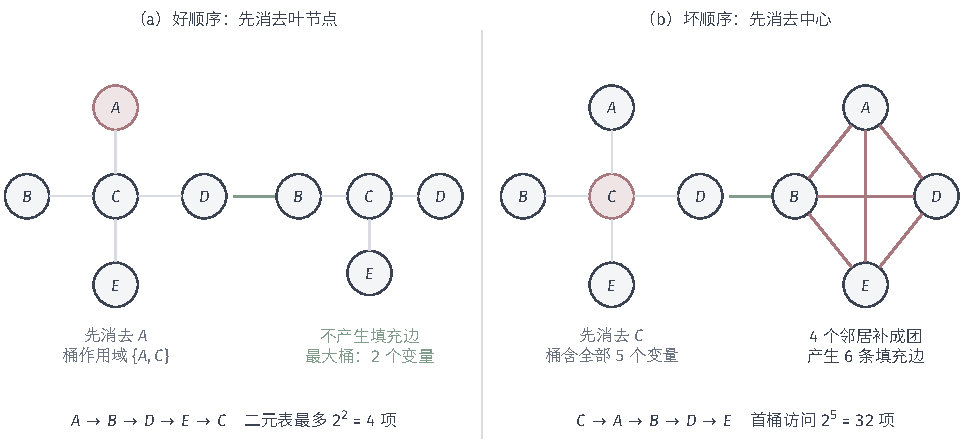
\includegraphics[width=163.153mm]{figures/09-probabilistic-graphical-models/02-inference/tikz/pgm-elimination-order-cost/figure.pdf}
  \caption{五节点二元星形图的两种消元顺序。（a）先消叶节点，每桶至多两个变量且没有填充边；（b）先消中心，首桶枚举$2^5=32$个配置，四个剩余邻居被补成团。红色节点是本步待消变量，红边是新填充边。两边比较稠密表算法的结构代价，最终数值答案保持相同。}
  \label{fig:pgm-elimination-order-cost}
\end{figure*}

要在真正计算函数值之前就预测每一步的表有多大，可以只根据“哪些变量同属一个因子”画出一张辅助图。构造\term{原始关系图}（primal graph）：把每个当前因子的输入节点两两相连，以图邻接记录同一局部函数中的共同坐标。证据代入后，按剩余实际作用域建图；有向条件表的家庭先形成团，再去掉已固定坐标。这个构造保留因子输入，所得图可以异于原DAG骨架。

有了原始关系图，就能直观地看到一次消元对结构的改变。

当前图中节点$i$的邻居记为$N(i)$。桶积使用$\{i\}\cup N(i)$，消去$i$后输出的作用域为$N(i)$，因此将这些剩余节点两两相连并删除$i$。其中新增的边称为\term{填充边}（fill edge），表示新函数的潜在共同作用域；特定参数仍可能使输出抵消或进一步分解。把该顺序产生的填充边全部保留，得到\term{诱导图}（induced graph）。

消元把内部变量的贡献保存到邻域函数。例如先消$H$，$\sum_h p(h\mid f)\ell_A(h,s)$仍以$f,s$为坐标，填充边$F-S$记录这个输出范围。对每组邻域状态，新表保存桶中子问题的完整汇总，后续直接读取它即可。图的填充说明需要保存哪些坐标，函数值说明每组坐标的数值贡献。

\begin{definition}[诱导宽度与树宽]
  \label{def:pgm-elimination-treewidth}
  对无向交互图$\mathcal{G}$的一条完整消元顺序$\pi$，令$N_t$为消去第$t$个节点之前、已经加入前面填充边后的剩余邻居集合。该顺序的\term{诱导宽度}（induced width）是
  \[
    w(\pi)=\max_t|N_t|.
  \]
  图的\term{树宽}（treewidth）定义为所有完整消元顺序中的最小诱导宽度：
  \[
    \operatorname{tw}(\mathcal{G})=\min_\pi w(\pi).
  \]
  宽度不包含本步被消去的节点，所以最大桶作用域的大小为$w(\pi)+1$。
\end{definition}

树宽给出能够达到的最小剩余邻域上界。森林可逐个消叶；含至少一条边时，其树宽为$1$。$d$节点完全图的首节点总有$d-1$个邻居，故树宽为$d-1$。这两个例子说明，节点数之外还需考虑局部作用域的重叠和可选顺序。

每个离散桶需访问多少状态，由变量基数共同决定。记$r_i=|D_i|$，定义作用域状态数
\[
  D(A)=\prod_{i\in A}r_i,\qquad D(\varnothing)=1.
\]
$D(A)$统计状态组合，集合$A$则指定变量。第$t$桶有$c_t$个因子，合并作用域$U_t=\{i_t\}\cup N_t$；稠密对齐、相乘及汇总使用$O(c_tD(U_t))$次标量操作，输出有$D(N_t)$项。完整保存乘积$\phi_t$需另有$D(U_t)$项工作存储。也可枚举每组$\bm{x}_{N_t}$，在$x_{i_t}$轴累加或取最大，把新增工作表缩至$D(N_t)$项；输入及其它未处理函数仍同时占用空间。

所有状态数至多$r$、输入因子数$m=O(d)$时，宽度$w$的完整顺序给出总运算上界
\begin{equation}
  T=O(d\,r^{w+1}).
  \label{eq:pgm-elimination-discrete-time}
\end{equation}
这个总界可以由各桶的代价逐项相加得到。宽度为$w$意味着$|U_t|\leq w+1$，所以每桶的状态数$D(U_t)\leq r^{w+1}$。每个因子只在首个收集它的桶中消耗，每步再产生一个新因子；即使计入孤立变量补入的单位因子，总处理出现次数仍为$\sum_t c_t=O(m+d)$。因此
\[
  \sum_t c_tD(U_t)
  \leq r^{w+1}\sum_t c_t
  =O((m+d)r^{w+1}).
\]
在$m=O(d)$条件下便得到式~\eqref{eq:pgm-elimination-discrete-time}；去掉这一假设时，上式的$d$相应换为$m+d$。此处按标量运算单位成本计，精确有理数位数的增长另属位复杂度。完整物化桶积的峰值为$O(r^{w+1})$，全部新因子及MPE回溯表可由$O(d\,r^w)$上界，实际同时存活部分可能较小。总空间还包括原输入，因而需分别报告输入、临时乘积及保留输出。

边缘查询只消去$R$，保留$Q$。若显式输出完整查询联合表，最后还需$D(Q)$项。设消元阶段的最大$|N_t|$为$w_R$，无消元步骤时取$w_R=0$。消元桶的状态数至多$r^{w_R+1}$，最终查询表则有$D(Q)\leq r^{|Q|}$项。为了用同一个指数上界同时容纳这两种计算，令$\bar w+1$至少等于$w_R+1$和$|Q|$，即将输出规模纳入指标：
\[
  \bar w=\max\{w_R,|Q|-1,0\}.
\]
式中的$|Q|-1$来自输出指数$|Q|$与宽度指数$\bar w+1$的对应，并不表示查询变量少算一个。$Q=\varnothing$时，输出仍是单项标量，$D(Q)=1$；无消元或空查询时再与$0$取最大，避免使用负宽度。在同一基数条件下，消元与最终表乘积的总时间上界为$O((m+d)r^{\bar w+1})$：前一部分沿用逐桶计数，后一部分在每组查询配置上读取全部剩余因子，其处理次数也不超过$O(m+d)$。输出空间为$D(Q)$项。分析显式输出时，也可预先把$Q$补成团并安排在顺序末尾。普通树宽在全部节点的顺序中优化，此查询则要求保留$Q$，两者的候选顺序集合不同。

两种常用启发式通过当前诱导图选择下一变量。\term{最小度启发式}（min-degree）取剩余邻居最少的节点，控制当前桶的变量数；\term{最小填充启发式}（min-fill）取邻居之间缺边最少的节点，试图减少后续填充。每步补边后重新计算这些指标，才能反映当前函数作用域。局部指标可给出可用顺序，但一般不保证全局最优；最小树宽排序在一般图上是NP难问题，通常先用启发式估计中间表规模，再决定是否执行精确消元\scite{pgm-koller2009}

基数不等时，较少变量也可能组成较大表。例如三个大基数变量的桶可能超过五个二元变量的桶：若前者每个变量都有$10$个状态，则需$10^3=1000$项，后者只需$2^5=32$项。\term{最小权重启发式}（min-weight）的一种约定据此比较新输出表项数，优先取$\prod_{j\in N(i)}r_j$最小的$i$，等价地比较$\sum_{j\in N(i)}\log r_j$。

若指标针对当前桶的枚举量，则比较$\sum_{j\in\{i\}\cup N(i)}\log r_j$，多计入待消变量的基数。加权填充还可对新增边$\{i,j\}$使用$r_ir_j$计分，它衡量新连接的成本，与前两种状态数指标不同。为得到候选节点的总分，记$\mathcal{E}_{\mathrm{new}}(v)$为消去$v$时必须补入的边，即当前邻域$N(v)$内尚未相连的无序节点对，并计算
\[
  s_{\mathrm{fill}}(v)
  =\sum_{\{i,j\}\in\mathcal{E}_{\mathrm{new}}(v)}r_ir_j.
\]
没有新增边时该和为$0$。这里$v$是候选消元节点，$i,j$是它的邻居，不能把$r_ir_j$误读为还要乘入$r_v$。

三个指标可能选择不同节点。例如一个$20$状态候选$v$有两个互不相连的二元邻居，其输出有$4$项，当前桶访问$80$项，填充分数为$4$。另一个二元候选$u$有三个已互相连成团的二元邻居，其输出有$8$项，当前桶访问$16$项，填充分数为$0$。按输出大小会先选$v$，按当前枚举量或本例填充分数则先选$u$。这些权重代理计算量，不表示概率。边缘MAP采用本章两阶段方案时，候选还需满足阶段限制：求和完成前，只在尚未消去的求和节点中选择；全部求和完成后，才对目标节点使用相同启发式。

高斯作用域的扩大增加矩阵维度及非零块。一次块消元消去$b$维、保留$a$维，对齐并累加$c_t$个稠密规范因子需$O(c_t(a+b)^2)$。式~\eqref{eq:pgm-elimination-schur}可通过分解与求解实现。正定主块允许写成Cholesky形式$\bm{J}_{B,B}=\bm{L}\bm{L}^{\top}$，其中$\bm{L}$为正对角的下三角矩阵。计算$\bm{W}=\bm{J}_{B,B}^{-1}\bm{J}_{B,A}$时，先前代求$\bm{L}\bm{Y}=\bm{J}_{B,A}$，再回代求$\bm{L}^{\top}\bm{W}=\bm{Y}$，便得到同一个$\bm{W}$，无需显式形成逆矩阵。对$\bm{h}_B$执行同样两次三角求解，得到一次项与常数项需要的向量$\bm{v}=\bm{J}_{B,B}^{-1}\bm{h}_B$。

这些运算也解释了各项成本。Cholesky分解$\bm{J}_{B,B}$需$O(b^3)$；块右端$\bm{J}_{B,A}$有$a$列，每列两次三角求解需$O(b^2)$，合计$O(b^2a)$；形成$\bm{J}_{A,B}\bm{W}$需$O(a^2b)$。一次项的$\bm{J}_{A,B}\bm{v}$与常数项的$\bm{h}_B^\top\bm{v}$不超过这些主操作的量级。核心更新因此使用
\begin{equation}
  T_{\mathrm{Gauss}}
  =O(b^3+b^2a+ba^2),\qquad
  S_{\mathrm{Gauss}}=O((a+b)^2).
  \label{eq:pgm-elimination-gaussian-cost}
\end{equation}
逐个消标量时$b=1$，对$a$邻居做二次规模更新，总消元典型代价为$O(\sum_t(|N_t|+1)^2)$，另计输入装配。总维度$q$的稠密高斯系统使用$O(q^3)$时间和$O(q^2)$空间，规模按矩阵维数增长。节点代表不同维度块时，成本比较需使用实际$a,b$。

\begin{table}[htbp]
  \centering
  \begin{tabularx}{\linewidth}{@{}lXX@{}}
    \toprule
    比较项 & 离散稠密表格 & 单个高斯规范形式\\
    \midrule
    作用域的表示 & 每种联合状态一项 & 二次项矩阵、一次项向量、常数\\
    合并因子 & 坐标对齐后逐项乘 & 坐标对齐后参数相加\\
    边缘消元 & 对被消去状态求和 & 配方积分与Schur补\\
    主要规模 & 基数乘积$D(U_t)$ & 矩阵块维度$a,b$\\
    填充的后果 & 新表可能指数增大 & 更多非零块与矩阵运算\\
    \bottomrule
  \end{tabularx}
  \caption{离散表与单高斯核的局部计算比较。前者以联合状态索引保存函数，后者以二次矩阵、线性向量和常数保存函数。右列对局部桶积分只要求被积分主块正定，局部输出本身可没有足够约束；所有剩余因子组合成完整查询核后，才以完整精度正定保证可归一化。含离散隐变量后可能增长的混合分量另需计数。}
  \label{tab:pgm-elimination-representation-cost}
\end{table}

边缘MAP在本章的通用算法中采用两阶段顺序，因而需要查询相关宽度。前面已经说明，作用域允许的某些交错顺序也结构有效，不能把“有效”直接等同于“两阶段”。不过，对标准结构有效的消元顺序，目标最后的同宽顺序仍然存在，所以把宽度优化限制到两阶段族不会漏掉这一消元族可达到的最小宽度。以$\Pi_{R\prec M}$记全部先排$R$、后排$M$的完整顺序，两组各自内部可任意排列，定义\term{受约束树宽}（constrained treewidth）为
\begin{equation}
  w_{\mathrm{c}}(\mathcal{G};R,M)
  =\min_{\pi\in\Pi_{R\prec M}}w(\pi).
  \label{eq:pgm-elimination-constrained-width}
\end{equation}
某条两阶段顺序的$w(\pi)$是该约束下的诱导宽度。候选集合是全部顺序的子集，所以最小值$w_{\mathrm{c}}\geq\operatorname{tw}(\mathcal{G})$。这个指标针对保证任意非负因子正确的两阶段稠密消元，计结构作用域成本；特定函数可交换算子的优势或其它MAP算法的时间下界属于不同分析对象。

执行一条已选两阶段顺序时，离散时间式~\eqref{eq:pgm-elimination-discrete-time}采用该顺序的实际宽度$w(\pi)$。采用最佳两阶段顺序才可用$w_{\mathrm{c}}$，得到$O((m+d)r^{w_{\mathrm{c}}+1})$上界；启发式顺序仍可能更宽。受约束树宽因此描述这组顺序可达到的最好结构上界。

以二元星形模型展示普通宽度与受约束宽度的差距。中心$X_0$连接$k$个叶$X_1,\ldots,X_k$，联合积为$p(x_0)\prod_{j=1}^k p(x_j\mid x_0)$。纯求和或MPE先消叶，每步仅一个邻居，普通树宽为$1$。若边缘MAP目标是全部叶，中心需先求和，两阶段算法的第一步为
\begin{equation}
  g(x_1,\ldots,x_k)
  =\sum_{x_0}p(x_0)\prod_{j=1}^{k}p(x_j\mid x_0).
  \label{eq:pgm-elimination-star-map}
\end{equation}
消中心后，$k$个叶成为同一函数的输入并补成团，所以受约束树宽为$k$。物化$g$需要$2^k$项，中心桶要枚举$2^{k+1}$个配置，而初始仅有$O(k)$张常数大小表。图~\ref{fig:pgm-elimination-constrained-star}显示$k=4$时的填充。

\begin{figure}[htbp]
  \centering
  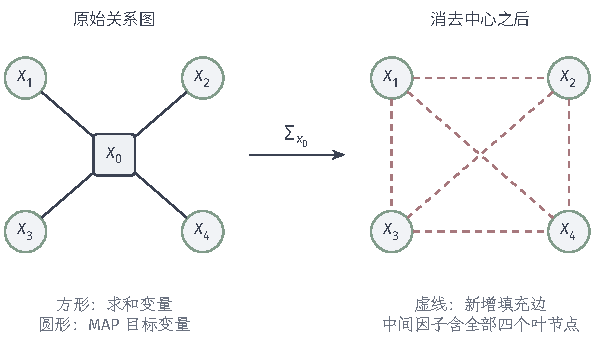
\includegraphics[width=100.651mm]{figures/09-probabilistic-graphical-models/02-inference/tikz/pgm-elimination-constrained-star/figure.pdf}
  \caption{四叶星形模型的边缘MAP消元。左图的目标是四个叶，中心$X_0$先求和；右图用虚线标出新叶间连接，记录四元输出作用域。MPE则允许先消叶，沿此顺序没有这些填充边。}
  \label{fig:pgm-elimination-constrained-star}
\end{figure}

特定参数可让式~\eqref{eq:pgm-elimination-star-map}的输出再次分解，其它算法也可利用这种结构。对仅按作用域操作的通用稠密消元，原图树宽$1$与查询受约束宽度$k$的差别却直接反映中间表增长。这解释了同一图上的边缘MAP为何可能比纯求和和MPE代价更大\scite{pgm-elimination-park2004}

\subsection{实现与适用边界}
\label{sec:pgm-elimination-implementation}

精确算法在数学上给出的是精确等式，但在计算机里用有限精度的浮点数执行时，等式可能变成带误差的近似；表很大、因子很多时这些误差还会累积。本小节讨论实现中必须处理的实际问题：表怎样按变量轴对齐、零值怎样稀疏存储、高斯矩阵怎样高效消元、连乘小数怎样避免下溢，以及什么时候精确VE根本不再可行。离散表的每一项需要以变量轴和状态编码定位，作用域信息随数值一起保存。相乘前按变量名对齐，或先转置再广播，可以使共享坐标确实表示同一状态。转置是在不改数值含义的情况下重排变量轴；广播则把缺失变量表示为长度$1$的轴，使该因子的值沿该变量的全部状态重复读取。例如将$\psi(f,h)$和$\eta(h,s)$相乘时，先统一为$(f,h,s)$轴顺序，分别用形状$(r_F,r_H,1)$和$(1,r_H,r_S)$的数组保存，再按共同的$h$索引读取并相乘，结果形状为$(r_F,r_H,r_S)$。

确定性约束产生的零项可用稀疏存储省去；消元后是否继续节省，则取决于新表非零项数。这里把函数取非零值的配置集合称为它的支持。求和会合并不同被消状态下的非零支持：若二元表仅在$(x,y)=(0,0)$和$(1,1)$处取$1$，其它项为零，则固定$x=0$和$x=1$时分别只支持一个$y$状态；求和$\tau(y)=\sum_x\psi(x,y)$后，两种$y$状态却都取$1$。原表只需保存两项非零值，输出的一元表已是稠密表。求和合并不同支持、填充扩大坐标范围，都可能令表变稠密，因此先估计峰值作用域，并在运行时记录非零项的实际增长。

高斯模型可用\term{稀疏Cholesky分解}（sparse Cholesky factorization）实现消元：将正定精度矩阵分解为三角因子，保存原非零项及新填充项。排序和符号分析先确定可能填充的位置，数值阶段再计算系数。这里的符号分析只读取非零模式，预测三角因子需要保存哪些位置；它不对概率公式作符号代数化简。例如消去一个同时连接$u,v$的标量节点时，Schur更新可能在原来为零的$(u,v)$精度块上产生新值，图中的填充边便对应这一新非零位置。相同稀疏模式可复用排序与符号结果；复用已有数值分解还要求矩阵值相同。

Schur式~\eqref{eq:pgm-elimination-schur}的逆矩阵运算可沿用前面的两次三角求解。积分常数需要的行列式也从同一分解读取：$\det(\bm{L}\bm{L}^{\top})=(\prod_j L_{j,j})^2$，且$L_{j,j}>0$，所以
\[
  \log|\bm{J}_{B,B}|=2\sum_{j=1}^{b}\log L_{j,j}.
\]
无需另求逆矩阵或先形成可能极大、极小的行列式，再取对数。

很小的权重连续相乘时，浮点数可能下溢。\term{对数域}（log domain）保存$\log\psi$，将因子乘积改为对数相加，零权重记为$-\infty$。MPE对这些和取最大值，保留同样的回溯索引。边缘查询仍需汇总所有状态，使用对数求和指数式实现这项操作：
\begin{equation}
  \log\sum_i\exp a_i
  =a_{\max}+\log\sum_i\exp(a_i-a_{\max}),
  \qquad a_{\max}=\max_i a_i.
  \label{eq:pgm-elimination-logsumexp}
\end{equation}
当$a_{\max}$有限时，减去它后至少一个指数为$1$，其余不超过$1$，避免直接对大数取指数。全体$a_i=-\infty$表示总权重零，此时直接返回$-\infty$，绕过无定义的无穷相减。若最终查询表处处零，归一化分母也为零，程序返回证据与模型不相容。

中途缩放因子也可控制数值量级。取一个与全部因子坐标无关的$s_t>0$，将$\tau_t$保存为$\widehat{\tau}_t=\tau_t/s_t$；记累计尺度$C_t=\prod_{j=1}^t s_j$，当前不变式相应为
\[
  C_t\prod_{\psi\in\widehat{\mathcal{F}}^{(t)}}\psi
  =\text{原始函数按已执行顺序聚合后的结果}.
\]
累计尺度以$\log C_t=\sum_{j=1}^t\log s_j$保存。条件分布的公共尺度最终抵消，而证据权重及最优绝对得分需恢复它。空作用域的标量因子同样影响原权重，必须明确它在累计尺度与当前因子积之间保存在哪里。本章选用的约定是：标量仍留在$\widehat{\mathcal{F}}^{(t)}$中，$C_t$只记录实际除去的$s_j$，不把同一个标量再次乘入$C_t$。例如当前另有标量$2$，把新因子$\tau$除以$3$后，恢复式为$3\times2\times(\tau/3)=2\tau$；若又把$2$乘入累计尺度而仍保留原标量，就会重复计入。

另一种等价实现是把正标量从因子集合取出，只向累计对数加入一次它的对数；这时累计尺度的记录还包括这些取出动作，不能再只记$\prod_j s_j$。两种约定不能混用。标量为零时，完整非负函数恒为零，应进入总权重零的处理分支，不能把零当作$s_t>0$的一部分取对数。

高斯核的可归一化性需要说明所用空间和测度。完整精度仅半正定、却仍在整个欧氏空间使用规范形式密度时，无二次约束方向的积分会发散。模型若限定在低维仿射子空间，应明确支持及子空间测度，在该空间上积分；伪逆和伪行列式本身不足以表达这些约定。理论正定但数值接近奇异时，检查条件数、变量尺度和分解残差以判断误差放大。对角扰动可以改善数值条件，却同时改动概率模型，应在采用时说明大小及影响。

最后说明精确VE的适用边界，以及多次查询时的复用。已知因子分解和明确查询后，可按预计中间作用域判断是否使用精确VE。离散表的高树宽或大受约束宽度可能耗尽内存；单高斯核按矩阵块维度增长，巨大块及填充也会带来高昂代价。相关信息无法全部保存时，第~\ref{chap:pgm-variational}章与第~\ref{chap:pgm-sampling}章分别通过变分和采样完成近似推断。

多次查询还涉及局部计算的复用。同一模型先问$F$再问$S$，从头消元会重复构造部分中间函数。模型与证据允许共享时，可缓存这些汇总，并在后续查询中读取或组合。判断一个缓存是否仍有效，需要记下它所依赖的原因子参数、已代入的证据值以及已经汇总的变量。相关参数或证据改变后，要重新计算受影响的缓存；若新查询需要某个已经被求和或最大化掉的变量，也不能直接从缓存恢复该变量的状态信息。沿本章原有$S,H$顺序得到的$\tau_S(h)$和$\tau_H(f)$都已消去$S$，因此不能直接拿来回答后续$S$查询。

保留两个目标坐标后，才可能供这两类查询共享。例如首次查询$F$时改为先消$H$，缓存
\[
  \eta(f,s)=\sum_h p(h\mid f)\ell_A(h,s).
\]
这张表所依赖的过热条件表、报警条件表及报警证据不变时，$F$与$S$查询分别使用
\[
  g_F(f)=p(f)\sum_s p(s)\eta(f,s),
  \qquad
  g_S(s)=p(s)\sum_f p(f)\eta(f,s).
\]
两式先给出各自的未归一化权重，再分别对全部$f$或$s$归一化得到后验。它们共享同一张没有消去$F,S$的$\eta$表，但先消$H$需要三变量桶，比原$S,H$顺序的首桶更大。单次查询的较小中间表与多次查询的复用机会由此形成实际权衡。第~\ref{chap:pgm-junction-tree}章据此组织消息与团树，减少重复工作；作用域本身很大时，其存储成本仍需承担。

\section{本章小结}
\label{sec:pgm-elimination-summary}

本章作为推断部分的开篇，把“模型给定后如何回答查询”落成一个可验证的精确算法。其主线可以用三句话概括。第一，故障后验可以直接从局部因子算出：代入报警证据，逐桶相乘并汇总非查询状态，再统一归一化；整个过程由一个不变式保证——当前乘积始终等于原函数对已消变量的聚合结果，所以局部替换与完整枚举给出相同答案。报警例的$p(F=1\mid A=1)\approx0.384111$把无故障过热、传感器失灵、误报等所有解释都汇总进分母，而MPE的$(F,H,S)=(0,1,0)$只选取单个联合最优配置，二者回答的是不同诊断任务。

第二，查询的类型决定汇总算子，也决定可用的消元顺序。边缘概率累加未知状态；MPE取最大值并保存选择、逆序恢复完整配置；边缘MAP先汇总非目标状态再选目标配置，求和与最大化的顺序一般影响答案。当目标角色限制了可用顺序后，受约束树宽可能远大于普通树宽，星形模型中“先对中心求和”会让所有叶补成团、生成多叶联合表，说明部分最优查询在结构上就可能比纯求和或MPE更贵。

第三，计算代价不由变量总数、而由消元顺序产生的中间作用域和所用函数表示共同决定。离散表按基数乘积保存状态组合，中间规模随诱导宽度指数增长；单高斯规范形式通过矩阵参数相加和Schur补解析更新，成本由矩阵块维度及填充决定。选择精确推断时，还需保证归一化合法，并控制浮点尺度与求解误差。只要中间函数能存下，VE就给出可逐步验证的精确结果；重复查询可进一步共享已算出的函数，而作用域过大时则需要额外的团树结构或明确改用近似——这正是后续章节的内容。

\paragraph{扩展阅读}
Koller与Friedman的教材从因子运算推导变量消除。书中不同顺序的例子可用于比较每桶的输入坐标、输出作用域及状态组合数，进一步理解中间函数为何比原节点总数更直接地决定成本\scite{pgm-koller2009}
